\documentclass[9pt,twocolumn,twoside]{pnas-new}
% Use the lineno option to display guide line numbers if required.

\templatetype{pnasresearcharticle} % Choose template 
% {pnasresearcharticle} = Template for a two-column research article
% {pnasmathematics} %= Template for a one-column mathematics article
% {pnasinvited} %= Template for a PNAS invited submission
\usepackage{cleveref}

\title{Biomechanical trade-offs in the pelvic floor constrain the evolution of the human birth canal}

% Use letters for affiliations, numbers to show equal authorship (if applicable) and to indicate the corresponding author
\author[a,1]{Ekaterina Stansfield}
\author[b]{Krishna Kumar} 
\author[a,c]{Philipp Mitteroecker}
\author[c,a,d,1]{Nicole D.S. Grunstra}

\affil[a]{Department of Evolutionary Biology, University of Vienna, Vienna, Austria 1090}
\affil[b]{Department of Civil, Architectural and Environmental Engineering, Cockrell School of Engineering, University of Texas at Austin, Austin, Texas 78712-0273, USA.}
\affil[c]{Konrad Lorenz Institute for Evolution and Cognition Research, Klosterneuburg, Austria 3400.}
\affil[d]{Mammal Collection, Natural History Museum Vienna, Vienna, Austria 1010.}

% Please give the surname of the lead author for the running footer
\leadauthor{Stansfield} 

% Please add a significance statement to explain the relevance of your work

% Please add a significance statement to explain the relevance of your work
\significancestatement{The relatively small human birth canal has arisen from an
	evolutionary trade-off between multiple antagonistic selective forces. We present evidence that a large pelvic floor is disadvantageous for maintaining continence and supporting the weight of the inner organs and the fetus through multiple finite element analyses of pelvic floor models varying in size and thickness. An increase in pelvic floor size led to a disproportionately large deflection as well as higher tissue stretches and stresses. Increased pelvic floor thickness considerably reduced
	deflection by increasing stiffness. However, as a side effect, it increases the intra-abdominal pressure necessary for childbirth, thus reflecting another evolutionary trade-off affecting not only the size but also the thickness of the pelvic floor.}

% Please include corresponding author, author contribution and author declaration information
\authorcontributions{All authors contributed to the conception and design of the research. ES created the FE models and ran the experiments. ES and KK analyzed the data. All authors critically interpreted the results and all authors drafted and critically revised the manuscript.}
\authordeclaration{Authors have no competing interests.}
\equalauthors{\textsuperscript{1} Co-corresponding Authors.  katya.stansfield\@univie.ac.at and nicolegrunstra\@gmail.com}
%\correspondingauthor{\textsuperscript{2}To whom correspondence should be addressed. }

% At least three keywords are required at submission. Please provide three to five keywords, separated by the pipe symbol

\keywords{pelvic floor $|$ human birth canal $|$ biomechanics $|$ evolutionary trade-off $|$ finite element modeling} 

\begin{abstract}
Compared to most other primates, humans are characterized by a tight fit between the maternal birth canal and the fetal head, leading to a relatively high risk of neonatal and maternal mortality and morbidities. Obstetric selection is thought to favor a spacious birth canal, whereas the source for opposing selection is frequently assumed to relate to bipedal locomotion. An alternative, yet under-investigated, hypothesis is that a more expansive birth canal suspends the soft tissue of the pelvic floor across a larger area, which is disadvantageous for continence and support of the weight of the inner organs and fetus. To test this ‘pelvic floor hypothesis’ we generated a finite element model of the human female pelvic floor and varied its radial size and thickness while keeping all else constant. This allowed us to study the effect of pelvic geometry on pelvic floor deflection (i.e., the amount of bending from the original position) and tissue stresses and stretches. Deflection grew disproportionately fast with increasing radial size, and stresses and stretches also increased. By contrast, an increase in thickness increased pelvic floor stiffness - i.e. the resistance to deformation - which reduced deflection but was unable to fully compensate for the effect of increasing radial size. Moreover, larger thicknesses increase the intra-abdominal pressure necessary for childbirth. Our results support the pelvic floor hypothesis and evince functional trade-offs affecting not only the size of the birth canal but also the thickness and stiffness of the pelvic floor.
\end{abstract}

\dates{This manuscript was compiled on \today}
\doi{\url{https://doi.org/10.1073/pnas.2022159118}}

\begin{document}

\maketitle
\thispagestyle{firststyle}
\ifthenelse{\boolean{shortarticle}}{\ifthenelse{\boolean{singlecolumn}}{\abscontentformatted}{\abscontent}}{}

% If your first paragraph (i.e. with the \dropcap) contains a list environment (quote, quotation, theorem, definition, enumerate, itemize...), the line after the list may have some extra indentation. If this is the case, add \parshape=0 to the end of the list environment.
\section*{Introduction}
\dropcap{H}umans are characterized by a close match (and occasional mismatch) between the dimensions of the maternal bony pelvis and fetal size. This tight fetopelvic fit leads to a comparatively difficult birth process in humans. Without medical intervention, fetopelvic disproportion often leads to maternal and neonatal death. Birth-related morbidities such as pelvic organ prolapse (i.e., the pathological descent of organs into or through the vagina or rectum) and incontinence affect millions of women worldwide, which can have serious social and health consequences~\cite{Arrowsmith1996-jn}. In western countries, a quarter to more than half of women report suffering from one or more pelvic floor disorders, with the reported prevalence of urinary incontinence ranging from 15\% to 69\% and of prolapse ranging from 6\% to 41\%~\cite{Lukacz2006-oz,Kenton2006-py,Lawrence2008-kg,Nygaard2008-ar}. Although their prevalence increases with age and parity, pelvic floor disorders are also common among young and nulliparous women~\cite{Lawrence2008-kg,Nygaard2008-ar,Dietz2005-to}. Understanding the evolutionary origins of obstructed labor thus is a pressing and highly debated challenge~\cite{Dunsworth2012-ip,Brown2013-pi,Wells2015-lo,Mitteroecker2016-bm,Grunstra2019-wq,Pavlicev2020-zl}.

Obstetric selection favoring a spacious birth canal is corroborated by the pronounced sex differences of pelvic dimensions in humans as well as in certain non-human primates and placental mammals~\cite{Grunstra2019-wq,Tague2005-os,Fischer2015-tu,Moffett2017-xv,DelPrete2019-ff}. However, there is a lack of consensus on the opposing selective forces that favor small pelvic dimensions. A narrow pelvis has long been argued to enable and benefit bipedal locomotion~\cite{Washburn1960-gm,Ruff1995-mz,Rosenberg2005-tl} but empirical evidence for this claim is equivocal~\cite{Gruss2017-bn,Warrener2015-tt,Whitcome2017-gh}. Abitbol (1988)~\cite{Abitbol1988-ir} first suggested that, in upright humans, a small bony birth canal contributes to the structural capacity of the pelvic floor to support the weight of the abdominopelvic organs and a large fetus as well as to withstand fluctuations in intra-abdominal pressure associated with physical activities (e.g., coughing, exercise) while maintaining continence~\cite{Brown2013-pi,Grunstra2019-wq,Pavlicev2020-zl}. The high frequency of incontinence and prolapse may thus result from the evolutionary conflict between a supportive pelvic floor and a birth canal capacious enough to pass a large baby. Clinical studies are equivocal in support of this `pelvic floor hypothesis’, where some found that women with mediolaterally broader pelves are more prone to develop incontinence and prolapse~\cite{Brown2013-pi,Sze1999-tb,Handa2003-fp}, while other studies failed to find such associations~\cite{Li2015-vk,Stein2009-fq,Handa2009-ri}. This incongruence presumably owes to the relatively limited morphological variation observable in modern populations and the presence of other risk factors that are unrelated to pelvic form. Apart from these correlational studies, the `pelvic floor hypothesis’ remains untested.

A certain level of pelvic floor deflection (i.e., the amount of bending from its original position), occurs during voiding of the bladder and rectum and is a normal part of urinary and fecal continence. Extensive deflection of the pelvic floor muscles is required during childbirth~\cite{Bitti2014-tv,Fernandez2015-rb,Schawkat2018-et,El_Sayed2017-sy}. The pelvic floor also helps support the weight of the gravid uterus, which is especially important during the late stages of pregnancy. Thus, any additional deflection as a result of a wider birth canal may be disadvantageous and would need to be counteracted by elevated resting (passive and continuous) muscle tone activity, requiring additional muscle tissue to maintain the same level of pelvic floor functionality. This, in turn, may again complicate childbirth. Note that even if the contribution of pelvic geometry to the development of pelvic floor disorders is small and of secondary clinical relevance, any such association would nonetheless constitute a selective pressure that affects pelvic evolution. Clinical evidence suggests that patients with incontinence or pelvic organ prolapse tend to have thinner pelvic floor muscles~\cite{Bitti2014-tv,El_Sayed2017-sy,Morkved2004-bi,Hoyte2004-qr}. Beyond this, however, little is known about how the geometry of the pelvic floor (and indirectly that of the bony pelvis) affects its displacement and supportive capacity.	

The deformation of the pelvic floor under pressure is influenced by multiple factors. In addition to material properties, the geometry of the pelvic floor also influences its \textit{stiffness}, i.e., the ability to resist deformation in response to an applied pressure, which in turn affects the pelvic floor deflection. A wider or a thinner pelvic floor has lower ``geometric stiffness,” i.e., stiffness resulting from pelvic floor geometry rather than from material properties (``material stiffness”), leading to a larger deflection. Hence, excessive deflection due to lower geometric stiffness of the pelvic floor can undermine its support function during normal day-to-day activities and contributes to pelvic floor disorders, such as incontinence and pelvic organ prolapse~\cite{Bitti2014-tv, Fernandez2015-rb, Schawkat2018-et,El_Sayed2017-sy}.

Here, we present the first biomechanical study to test the pelvic floor hypothesis using a series of finite element (FE) analyses. We investigate the effect of variation in pelvic floor surface area and thickness on the amount of pelvic floor deflection. To this end, we created a model that reflects the main features of pelvic floor shape (\cref{fig:pelvic-floor}) and which, unlike clinical FE models~\cite{Martins2007-jn, Noakes2008-ee, Parente2008-ts,Cosson2013-ss,Jing2012-uu,Mayeur2016-qi, Silva2017-uz,Gordon2019-zl}, covers all of the unsupported surface of the pelvic floor. This approach allowed us to vary the radial size and thickness of the pelvic floor within and also beyond the size ranges observable in modern humans while keeping all else constant. Under the pelvic floor hypothesis, we expect that a more spacious pelvic canal (and thus a larger pelvic floor surface) leads to larger pelvic floor deflection. Furthermore, based on the engineering principle that material with larger stiffness deforms less, we expect that a thicker pelvic floor shows reduced deflection due to less tissue stretch (i.e., the ratio of the deformed final length over original length) and stress (i.e., force per unit area).

Like any muscle tissue, the pelvic floor behaves as a hyperelastic material with a nonlinear relationship between stresses and stretches~\cite{Humphrey2003-rb}. This implies that beyond a certain level of stretch the stress undergoes a considerable nonlinear increase towards the failure strength (the point at which the material will rupture), which can have fatal consequences for pelvic floor functioning. We therefore also study how pelvic floor geometry influences the levels of stresses and stretches, which in turn affect the displacement in response to pressure.  

When idealizing the pelvic floor as a circular linear-elastic membrane with equal thickness, the deflection under a given pressure can be computed analytically using the Airy stress function (see SI Appendix). The analytical solution demonstrates that membrane deflection increases nonlinearly (as a cubic polynomial) with an increase in the radius. However, for a radial size range of -2 to +7 standard deviations (SD) and the material properties considered in this study, the relationship between deflection and radius is approximately linear (SI Appendix, Fig. S1). By contrast, the deflection increases linearly when both the radius and the thickness of the membrane increase proportionately for all size ranges (SI Appendix, Fig. S1). Under these highly idealized conditions, the analytical solutions clearly support the pelvic floor hypothesis. The pelvic floor, however, is a complex three-dimensional structure and biomechanical behavior of muscles is nonlinear~\cite{Humphrey2003-rb}. Hence, we went beyond this analytical approach by using 3D FE models that more realistically represent pelvic floor anatomy (\cref{fig:pelvic-floor}). To quantify the impact of pelvic floor area and thickness on pelvic floor displacement and local tissue stress, we varied the surface area and thickness of a ``base model” with average anteroposterior (AP) length and mediolateral (ML) width and average thickness (see Materials and Methods). Importantly, we varied pelvic floor surface area and thickness beyond the normal range of human variation, which enabled us to observe how pelvic floor deflection is affected by `extreme’ phenotypes that have been selected against by natural selection and thus cannot be observed in modern populations.

\section*{Results}
\subsection*{Displacement scales disproportionately with pelvic floor radius}
To quantify the effect of bony pelvic canal size on the mechanical response of the pelvic floor, we varied the surface area of the pelvic floor while keeping its transverse shape (the ratio of AP length to ML width) and thickness constant. Using data from DelPrete~\cite{DelPrete2019-ff}, we constructed 22 different pelvic floor models by changing the transverse radii of the base model by increments of 0.5 or 1 SD of within-population variation~\cite{DelPrete2019-ff}. The models ranged from -4.2 to +7 SD in radial size (SI Appendix, Tab. S2). We expressed the transverse size of the pelvic floor, $R$, as the average radius (square root of the surface area of the model), divided by the average radius of the base model. Hence, the base model has $R$=1, which corresponds to the average size in the data of DelPrete~\cite{DelPrete2019-ff}. A change of approximately 0.08 in $R$ corresponds to a change of 1 SD in both AP and ML radii. We applied a pressure of 4 kPa to the superior surface of the model, which is within the range of intra-abdominal pressures associated with typical daily activities and exercises (see Materials and Methods). We quantified deflection by the displacement responses measured in two regions in the midsagittal plane, corresponding to the anterior and posterior anatomical compartments of the pelvic floor (see~\cref{fig:pelvic-floor} and Materials and Methods). 

\begin{figure}%[tbhp]
\centering
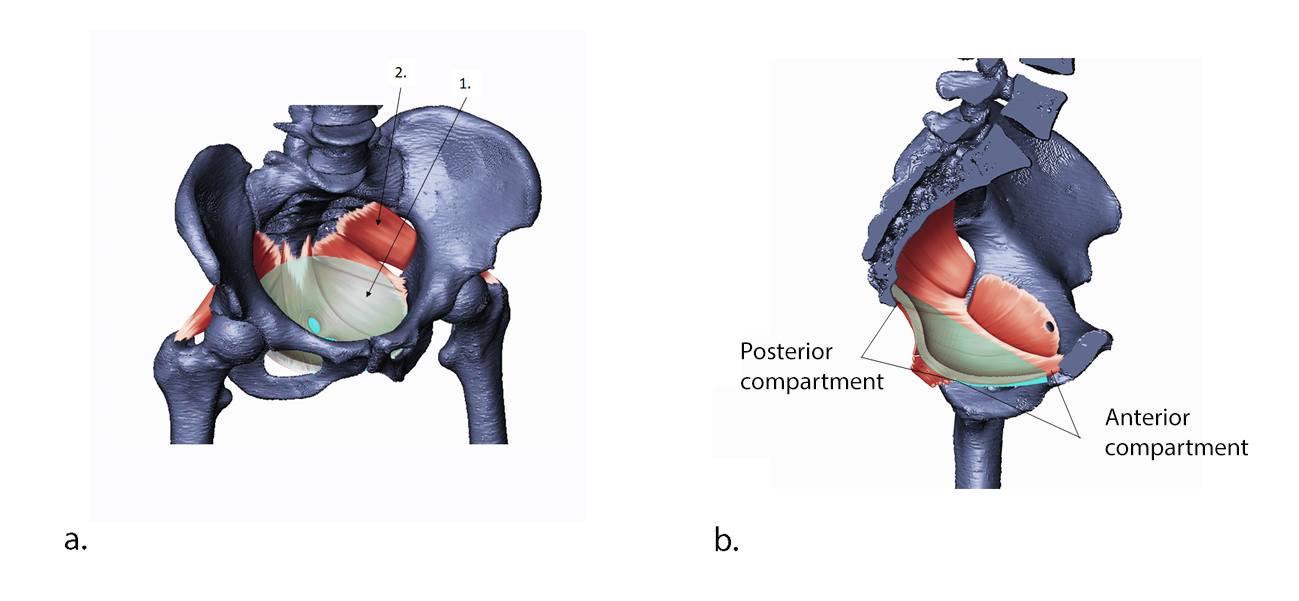
\includegraphics[width=\linewidth]{figs/fig1}
\caption{The pelvic floor is a system of muscles and connective tissue spanning the bony pelvic canal. (a) The model (``1,” transparent cyan) is shown superimposed on the pelvic floor muscles (``2,” red) and spans the part of the pelvic floor unsupported by bony structures. (b) Sagittal cross-section view showing the fit of the model superimposed on human female anatomy.}
\label{fig:pelvic-floor}
\end{figure}

For the idealized circular membrane, the analytical solution predicted an almost linear increase of displacement with the radius within the domain of $R$ ranging from 0.85 to 1.55 (\cref{fig:radius}). For the FE model, however, the pelvic floor showed a strong nonlinear increase in the displacement with $R$ in the anterior compartment and a bi-linear displacement in the posterior compartment (\cref{fig:radius}a). Furthermore, observing the displacement profiles of the model (SI Appendix, Fig. S2) reveals that for small and intermediate pelvic floors the displacement in the anterior and posterior compartments was localized to those regions, whereas for very large pelvic floors (approx. +3 SD and above), displacements impacted the entire model, resulting in a substantial increase in the overall deflection (\cref{fig:radius}a).  
Both the stretch and average Von Mises stress (a representative value of different stress components used to determine the maximum possible distortion of a material) increased with pelvic floor radius. For very small pelvic floors ($R<0.8$), the increase was very steep, showing that the effect of geometric constraints on stress and stretch are strongest for very small radial dimensions (\cref{fig:radius}b, c). The rate of increase in stretch in the anterior region was 12.3 times higher than in the posterior compartment (\cref{fig:radius}c). For all models and both compartments, stress and stretch were within the linear region of a hyperelastic stress-stretch relationship for the applied pressure of 4 kPa (SI Appendix, Fig. S3).

\begin{figure*}
\centering
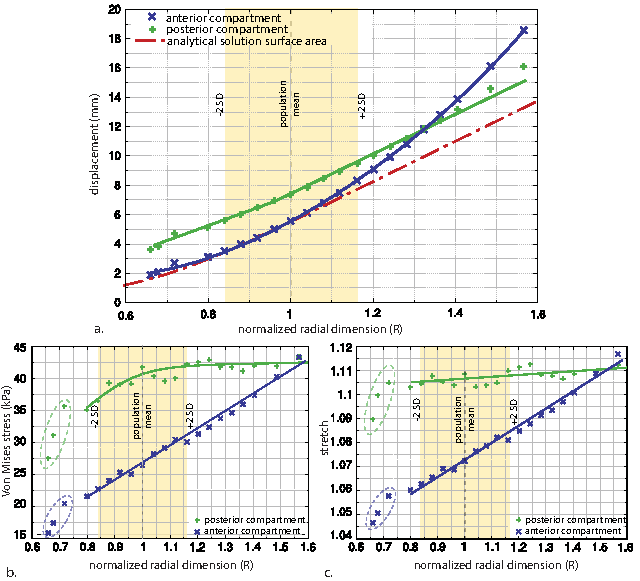
\includegraphics[width=.8\textwidth]{figs/fig2}
\caption{The effect of variation in the standardized pelvic floor radius, $R$, on (a) absolute pelvic floor displacement, (b) Von Mises stress, and (c) stretch. $R$ is
expressed as a multiple of the dimension of the base model. An $R$ of 1 equals the female population mean size, and ∼95\% of this population falls within the
range of $R$ from 0.84 to 1.16 ($\pm2$ SD). Pelvic floor thickness and pressure were kept constant (6 mm and 4 kPa, respectively). Displacement, stress, and stretch
were measured separately for the anterior and posterior compartments (blue “x” and green “+” symbols, respectively) as well as for the analytical solution
applied to a circular membrane (red dashed line). For intermediate pelvic floor dimensions ($0.8 < R < 1.1$), the anterior compartment showed an approximately
linear increase in displacement with a rate similar to that of the analytical solution, whereas it exhibited a substantial nonlinear increase in displacement
for larger than average pelvic floors. The displacement in the posterior compartment increased at a slightly slower rate than the analytical solution
until $R = 0.95$. Thereafter, the increase in posterior displacement was similar to that of the analytical solution and exceeded that for very large sizes ($R > 1.4$).}
\label{fig:radius}
\end{figure*}

\subsection*{Increased pelvic floor thickness reduces displacement} 
To study the effect of pelvic floor thickness on displacement, FE analyses were performed on multiple models with constant AP length and ML width but a thickness varying from 1 mm to 12 mm. An increase in thickness from 1 mm to 3 mm was found to strongly reduce the amount of displacement due to an increase in geometric stiffness, whereas beyond 3 mm the influence of an increase in geometric stiffness was less pronounced and the displacement decreased more gradually (\cref{fig:thickness}a). Similar behavior was observed for Von Mises stresses as thickness increased (\cref{fig:thickness}b). For thicknesses larger than 10 mm, an increase in thickness had little effect on the displacement response although stresses did decrease further.

\begin{figure*}
\centering
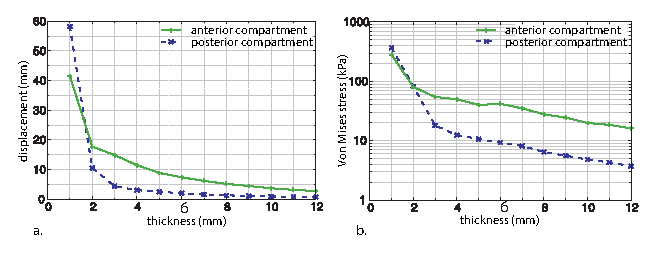
\includegraphics[width=.8\textwidth]{figs/fig3}
\caption{The effect of varying thickness and constant surface area ($R = 1$) and pressure (4 kPa) on (a) pelvic floor displacement and (b) Von Mises stress. For
thicknesses of 1 to 3 mm, the pelvic floor deflected most strongly (up to 60 mm), whereas beyond a thickness of 3 mm, displacement decreased more
gradually (a). Similar behavior was observed for stresses (b). The range of 1 to 12 mm roughly corresponds to the variation in thickness across the pelvic floor
and among individuals reported in the literature (SI Appendix, Table S1). The thickness of the base model is 6 mm.}
\label{fig:thickness}
\end{figure*}

\subsection*{Displacement scales disproportionately with the radius when thickness is increased proportionately}
In the above models, we separately varied the area and the thickness of the pelvic floors. Although it is unknown how pelvic floor thickness scales with surface area in humans, it is likely that pelvic floors with larger surface areas also tend to be thicker. Therefore, we repeated the analyses and varied thickness proportionately to the square root of the surface area.
The analytical solution for a circular membrane predicted a linear increase of displacement with a proportional increase in both radius and thickness. For the FE models, pelvic floor displacement also increased with $R$, but not in a simple linear way (\cref{fig:isometry}a). A transition in the displacement behavior occurred at $R=0.95$, where both anterior and posterior displacements started to increase considerably faster with size than observed for smaller pelvic floors. For the anterior compartment, the rate of increase was more than twice as high compared to that in the posterior compartment, with the latter following the same behavior as the analytical solution. However, for very large pelvic floors (approximately at $R>1.4$) displacement of the anterior compartment exceeded the displacement of the posterior compartment (\cref{fig:isometry}a), which coincided with the transition of localized anterior and posterior displacements to a more global displacement (SI Appendix, Fig. S4). Von Mises stress and stretch tended to remain almost unchanged in the anterior compartment (\cref{fig:isometry}b and \cref{fig:isometry}c), whereas the posterior region showed a strong decline in both stress and stretch. The stress-stretch relationship for each model was still in the linear portion of the expected stress-stretch curve (SI Appendix, Fig. S5).

\begin{figure*}
\centering
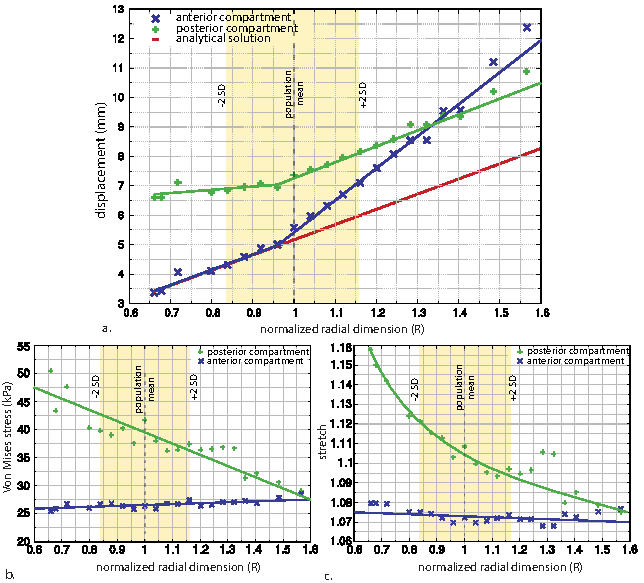
\includegraphics[width=\textwidth]{figs/fig4}
\caption{The effect of proportional variation in pelvic floor radius and thickness at constant pressure (4 kPa) on (a) pelvic floor displacement, (b) Von Mises
stress, and (C) stretch. Here, $R$ and thickness were increased by the same fraction. An $R$ of 1 equals the female population mean radial size, and ∼95\% of this
population falls within the range of $R$ from 0.84 to 1.16 ($\pm2$ SD). Displacement, stress, and stretch were measured separately for the anterior and posterior
compartments (blue ``x” and green ``+” symbols, respectively) as well as for the analytical solution applied to a circular membrane (red dashed line). For
smaller than average pelvic floors ($R < 0.95$), the displacement in the anterior compartment increased linearly at a rate equal to that observed for the analytical solution, whereas the displacement in the posterior compartment remained almost unchanged between 6.5 mm and 7 mm (a).}
\label{fig:isometry}
\end{figure*}

\subsection*{The 3D shape of the pelvic floor affects its mechanical response}
To explore how 3D shape (i.e., the inverted dome-like shape of the pelvic floor) affects the stress-stretch relationship of the FE model, we compared the stress-stretch response of the base model against a uniaxial tension test of a rectangular block of the Mooney-Rivlin material (see Materials and Methods). In a uniaxial tension test of an isotropic Mooney-Rivlin material with pelvic floor tissue properties, Silva and colleagues observed a linear increase in stresses with increasing stretch~\cite{Silva2017-uz}. However, deviations from this simple block geometry are likely to alter the stress-stretch relationship. We thus evaluated the stress-stretch relationship of our 3D FE base model and found that at lower stresses pelvic floor behavior resembled that of the uniaxial tension case, whereas for stretches higher than 1.11 the pelvic floor must be subjected to considerably higher stresses (i.e., pressures) to obtain the same stretches as under the uniaxial condition (\cref{fig:stress-strain}). In other words, at lower stretches ($<1.11$) material properties of the pelvic floor dictate its deflection, whereas at higher stretches, the 3D shape of the pelvic floor - which is different from block geometry - begins to dominate pelvic floor deflection.

\begin{figure}
\centering
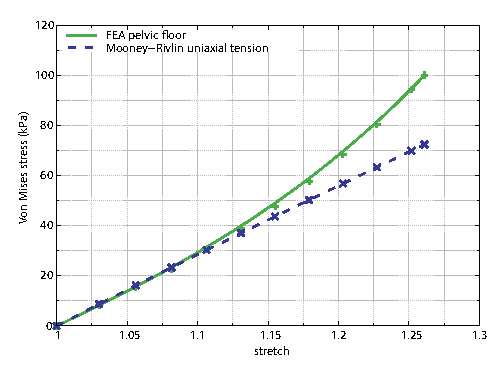
\includegraphics[width=\linewidth]{figs/fig5}
\caption{Stress–stretch behavior of the pelvic floor finite element model with
average dimensions (green) compared with the analytical Mooney–Rivlin
relations for uniaxial tension using material parameters based on continent
women (blue dashed). The model was subjected to a pressure of 15 kPa. The
stress–stretch relationship in the FE model clearly deviates from the uniaxial
linear response and shows a nonlinear relation for a stretch higher than 1.11
and a corresponding Von Mises stress higher than 30 kPa.}
\label{fig:stress-strain}
\end{figure}

\section*{Discussion}
Here we modelled the biomechanical behavior of the human pelvic floor for a range of different surface areas and thicknesses using a finite element approach. To our knowledge, this was the first time such an approach was used to explore what could be one of the primary causes of the``obstetrical dilemma" in modern humans. The analytical solution for an idealized circular membrane predicted an approximately linear increase of deflection with increasing radial dimensions above -2 SD, all else equal. But a more realistic finite element model showed that the deflection of the pelvic floor (expressed as the displacement in the anterior and posterior compartments) increased even faster with the radial dimensions than predicted by the analytical solution. We also showed that, for a given surface area, an increase in pelvic floor thickness caused a decrease in displacement. However, when increasing the thickness of the pelvic floor proportionately with its radius we observed only an incomplete compensation of the displacement. The overall deflection still increased faster with pelvic floor size than predicted by the analytical solution, which highlights the effect of three-dimensional pelvic floor geometry and nonlinear material response on its displacement behavior.
Surface area and thickness of the pelvic floor also affected tissue stresses and stretches in response to load, which can contribute to injuries and rupture of pelvic floor tissues~\cite{Humphrey2003-rb,Willis2002-eo}. Stress and stretch in the pelvic floor (especially in the anterior compartment) increased strongly with the radius and decreased with pelvic floor thickness. In small and intermediate pelvic floors, displacements and stresses in the anterior and posterior compartments were localized and constrained by the additional geometric stiffness afforded by small radial dimensions. For larger pelvic floor sizes, the localized displacements transitioned into global displacements (SI Appendix, Fig. S2), which severely increased deflection.
These outcomes are consistent with medical studies reporting that pelvic floor disorders, such as incontinence and pelvic organ prolapse, are more frequent in women with mediolaterally wider bony pelves (controlling for body size, age, and parity)~\cite{Brown2013-pi,Abitbol1988-ir,Sze1999-tb}. Taken together, this implies that an increase in the unsupported length of the pelvic floor muscles and fascia results in a decrease in its supportive capacity. The finding that increased thickness buffers against pelvic floor displacements also corresponds well with clinical reports of reduced thickness of the levator ani (the main group of pelvic floor muscles) in individuals with urinary or faecal incontinence and prolapse~\cite{Handa2009-ri,Schawkat2018-et,Wijma2007-hh}. 
Other studies, however, reported no association between the prevalence of pelvic floor disorders and bony pelvis size~\cite{Handa2003-fp, Stein2009-fq} or pelvic floor thickness~\cite{Yasar2019-ga}. This likely owes to the complex etiology of pelvic floor disorders and the small range of variation in the dimensions of the birth canal observable in modern human populations~\cite{Athanasiou2007-qg,Grabowski2013-ze}. As a result, other factors have a relatively stronger influence and perform as better clinical predictors of pelvic floor disorders, such as comorbidities, vaginal delivery, and tissue properties. Moreover, the female pelvis continues to remodel during adulthood, which further confounds comparisons of pelvic dimensions across different ages~\cite{Grabowski2013-ze,Ricklan2020-bs,Huseynov2016-qg}. Our FE models circumvented these complications by controlling for variation related to such factors and by investigating a broader range of pelvic floor size variation than is commonly observed in a modern human population. 
Comparing the 3D FE model with the uniaxial test on Mooney-Rivlin model revealed that stresses start to deviate from the linear response of the uniaxial test at a stretch value of ~1.11 (\cref{fig:stress-strain}). Unlike the rectangular beam in Silva et al. (2017)~\cite{Silva2017-uz}, our FE model has an inverted-dome-like structure (shell). This 3D shape contributes to an increase in stiffness and reduces its deflection. It thus requires substantially higher pressures, as occurring during vaginal birth, to cause stretches above 1.11 due to the non-linear stress-stretch relationship. This stress-stretch relationship also implies an ideal pelvic floor thickness of 6-10 mm. For these thicknesses, the Von Mises stresses in both the anterior and posterior region are below the critical value of 40 kPa (\cref{fig:thickness}), above which the stress-stretch relationship shows a significant non-linear response (\cref{fig:stress-strain}).
Our results clearly support the pelvic floor hypothesis of pelvic evolution~\cite{Mitteroecker2016-cd}. The evolution of a wider pelvic canal would have led to larger deflection of the pelvic floor and potentially also to higher stretches and stresses within the pelvic floor tissues, all of which predispose to pelvic floor dysfunction. Dysfunction of the pelvic floor can result from mechanical failure (i.e., rupture) of pelvic floor tissues or from the inability to perform its support function, i.e., the inability to support internal organs and their function or exceed a threshold value of deformation. Whereas rupture of pelvic floor muscle only happens at high stresses (440 ± 220 kPa along the direction of the fibre52), performance-based failures are more common. For instance, those leading to organ prolapse, incontinence, or insufficient support of a gravid uterus during pregnancy due to excessive deformation, resulting from, e.g., reduced (geometric or material) stiffness. The higher risk of impaired pelvic floor function in women with a large pelvic canal has thus imposed natural selection against a more spacious birth canal over the course of human evolution.  This selection for a small, supportive pelvis counteracts the obstetric selection for a spacious birth canal, giving rise to the ``compromise morphology” of the pelvis observable today.

But we also found that a thicker pelvic floor partially compensates for increased deflection and stress resulting from a large pelvic canal. A complete compensation, however, would require a disproportionate increase of thickness with the radial dimensions of the pelvic floor. So why did evolution not go down this route and compensated the biomechanical disadvantage of a large pelvic canal by a thicker pelvic floor? Our results provide one explanation. While additional muscle tissue would be beneficial for continence and supporting the visceral organs and fetus during pregnancy, it is likely disadvantageous for childbirth and possibly also defecation. Thicker muscle tissue requires higher pressures in order to undergo the same amount of deformation as thinner tissue (\cref{fig:thickness}b). During the second stage of labor, when the fetal head descends through the birth canal, the pelvic floor muscles stretch up to more than three times their original length~
\cite{Kuthe2016-rx,Lien2004-gj}. The average maximum intrauterine pressure that women produce during this stage of labor is around 19 kPa~\cite{Li2008-zh}, which presumably is (near) the upper limit that women are able to produce. In our study, we observed a maximum stretch of $\sim 1.26$ at 15 kPa pressure for a 6-mm thick pelvic floor (\cref{fig:stress-strain}). Women with much thicker pelvic floors would need to produce substantially higher forces during labor to acquire similar levels of deformation for successful delivery (despite the change in pelvic floor material properties during the late stages of pregnancy that afford higher flexibility~\cite{Rempen1991-ru}). Indeed, an FE simulation of the second stage of vaginal delivery showed that the relatively thick levator ani muscles of an athlete required a 45\% increase in peak force to expel the fetal head through the pelvic floor compared to a non-athlete with a thinner pelvic floor~\cite{Lien2004-gj}. For women to produce substantially higher intra-abdominal pressures, however, adaptations to diaphragm, uterine and abdominal muscle strength are required, which may be similarly evolutionarily constrained. This situation thus illustrates the presence of another functional and evolutionary trade-off in the human pelvic floor: not only the transverse dimensions but also the thickness of the pelvic floor has functionally opposing outcomes with regard to pregnancy and childbirth. 
Under such evolutionary trade-off dynamics, a trait evolves a compromise distribution that maximizes mean population fitness. If the opposing selective forces are of similar strength, the evolved population mean of the trait is expected to resemble the trait value with maximal individual fitness, i.e., the functionally ``optimal” trait value~\cite{Li2010-bb}. In the case of an asymmetric fitness function, i.e., if selection in one direction (e.g., towards a larger pelvic canal) is stronger than that in the other direction, the evolved population mean is expected to deviate somewhat from the functional optimum (in this case towards a larger canal size)~\cite{Mitteroecker2016-bm,Arnold2001-aj}. Within the limits imposed by the simplifications of our models, our results reflect these evolved compromises surprisingly well. Pelvic floor thicknesses below 3 mm resulted in significant stresses, whereas thicknesses beyond 10 mm did not considerably reduce stress and displacement any further but could aggravate parturition. These ``ideal” thicknesses between 6 mm and 10 mm correspond well with pelvic floor (specifically pubococcygeus muscle) thicknesses reported for continent, non-prolapsed women~\cite{El_Sayed2017-sy,Mayeur2016-qi,Wijma2007-hh}. Not only the thickness but also the average transverse size of the pelvic floor coincided well with a functional optimum: the increase in deflection with the radius was considerably faster for larger than average pelvic floors compared with pelvic floors smaller than the population mean. Even when pelvic floor thickness was scaled proportionately with the average radius, some trade-off was shown by the two compartments of the model. The displacement in the posterior region remained almost unchanged for $R<1$ but increased at the same rate as the analytical solution for larger than average sizes. The displacement of the anterior compartment, by contrast, showed the same rate as the analytical solution for smaller than average sizes and increased more strongly for $R>1$. The ``optimal” compromises between both the size of the pelvic canal and the overall pelvic floor deflection as well as between anterior and posterior pelvic floor displacements thus concur surprisingly well with the observed population mean ($R=1$), as expected for an approximately symmetric fitness trade-off.
The `pelvic floor hypothesis’ is one of several proposed explanations for the evolution of the relatively narrow birth canal in humans. Adaptations of human body form to bipedal locomotion, thermoregulatory demands, and the competing energy needs of the mother and the fetus are likely to have influenced pelvic dimensions as well~\cite{Dunsworth2012-ip,Grunstra2019-wq,Pavlicev2020-zl,Washburn1960-gm,Ruff1995-mz,Rosenberg2005-tl,Urban2013-ll}. Our simulation study allowed us to demonstrate that - independent of all these other factors - the biomechanical constraints imposed by the pelvic floor are likely to have played an important role in human pelvic evolution.

\section*{Materials and Methods}
The aim of this study was to understand the influence of pelvic floor surface area and thickness on its displacement response. Hence, to account for a wide range of geometric parameters and exclude the influence of potentially confounding factors (e.g., active muscle contraction, trauma), we idealized the pelvic floor geometry as a 3D oval hammock of uniform thickness transversely suspended in the midplane of the bony pelvic canal (\cref{fig:pelvic-floor}).
\subsection*{3D geometry}
\subsubsection*{Morphology}
A 3D pelvic floor model was created to represent the muscles and fibrous tissue, which support the internal organs in the transverse midplane of the pelvis: between the pubic bone and the coccyx anteroposteriorly, and between the ischial spines mediolaterally. Anatomically, this area is occupied by the levator ani muscles and urogenital diaphragm as well as the perineal membrane and tissues of the urethral sphincter, vagina, and rectum. The levator ani originates at the pubic bone and arcus tendineus and is responsible for the support of the abdominal viscera and urinary and fecal continence (see SI Appendix, Fig. S6). 
We based the thickness of our idealized pelvic floor on that of the pubococcygeus part of the levator ani, as this is the part of the pelvic floor that is roughly perpendicular to the vagina and pelvic organs and carries most of the load. Its thickness has been reported to differ between patients with and without medical conditions~\cite{Morkved2004-bi,Mayeur2016-qi,Wijma2007-hh}. Based on published data for levator ani thickness (see SI Appendix, Tab. S1), we used an average uniform thickness of 6 mm for our idealized pelvic floor model, which also matches the thickness reported in the dMRI study of living participants 40 against which we validated our FE model. 
\subsubsection*{Model dimensions and fit}
A CAD model of the pelvic floor was created in SOLIDWORKS © 1995-2019 Dassault Systémes. The anteroposterior diameter of the model corresponds to the distance from the inferior point at the pubic symphysis to the penultimate vertebra of the coccyx. The mediolateral diameter was taken between the ischial bones at the points of muscle insertion on the ischial spines. The superoinferior depth of the puborectalis sling was taken as 25 mm, the average value measured on several whole-body CT scans of adult human females from the New Mexico Decedent Image Database collection 60. The fit of the pelvic floor model inside the bony pelvis is shown in (\cref{fig:pelvic-floor}). 
To build FE models of different surface areas, we used means and standard deviations reported in the literature for the relevant anteroposterior and mediolateral pelvic floor dimensions, represented by the anteroposterior outlet and bispinous diameters measured on bony pelves of a large sample of modern human female skeletons of European descent 16. An examination of three whole-body NMDID CT scans 60 and five MRI scans from the UK Biobank database revealed that the mediolateral distance between the insertion points of the levator ani muscles on the ischial spines was approximately $110\%$ of the same distance between the tips of the bony spines (i.e., bispinous diameter). We, therefore, augmented the average bispinous diameter reported by DelPrete 16 by $10\%$. We created a ``base model” with the mean pelvic floor dimensions, namely anteroposterior and mediolateral radii of 56 mm and 53 mm, respectively, and a thickness of 6 mm.
\subsection*{Finite element model and its validation}
\subsubsection*{FE Model}
The pelvic floor CAD geometry was discretized using more than 110,000 elements with an average element size of 1.28 mm. The 10-noded tetrahedral elements with quadratic shape functions were used to discretize the model. An implicit solution scheme using FEBio 61 was adopted to solve the quasi-static loading problem. The boundary conditions involved constraining the mobility of the nodes of the elements along the top rim to zero in all three directions (X, Y, Z), and were identical across models. Constant pressure from above was applied as an equivalent normal force to the entire superior surface of the mesh. To attribute differences in displacement, stresses, and stretches of the pelvic floor to variation in the geometric parameters of interest, we kept the material properties the same across all experiments. 
\subsubsection*{Material properties}
Although our study required the design of a pelvic floor model with a different geometry than previous patient-specific models, we assigned material properties to our model as determined in previous work35,40. Specifically, we follow Silva et al.40, who obtained material parameters by comparing simulated pelvic floor displacement against recorded displacement during dynamic Magnetic Resonance Imaging (dMRI), when patients were asked to perform a straining, or Valsalva, maneuver. We adopted an isotropic Mooney-Rivlin constitutive law to represent pelvic floor tissues with the following parameters: c$_1$=26 kPa, c$_2$=14 kPa 40, and the bulk modulus, K = 1000 kPa to reflect the near-incompressibility of the material 61.
\subsubsection*{Model Validation}
The FE base model developed in this study was validated by comparing the displacements against those observed in the dMRI data of a pelvic floor subjected to a pressure of 4 kPa 40. The individual displacement components in the FE model were in good agreement with the measured dMRI data and within one standard deviation reported by Silva et al. 40 (SI Appendix, Fig. S7). 
\section*{Experiments}
Four experiments were carried out to investigate the structural response of the pelvic floor under different geometric conditions. The pelvic floor surface area and thickness varied beyond the range of typical pelvic floor geometry observed among modern human females, enabling us to observe the deflection response for pelvic floor sizes that have presumably been removed by natural selection during human evolution. 
\subsection*{1. Scaling of pelvic floor displacement with radius.} To investigate the dependence of pelvic floor displacement on radial dimensions, we created 21 additional FE models whose anteroposterior and mediolateral dimensions varied jointly from -4.2 SD to +7 SD of the base model’s radii (SI Appendix, Tab. S2). Hence, all 22 models had approximately the same two-dimensional (transverse) shape of the pelvic floor, with a constant thickness of 6 mm, and all were subjected to a pressure of 4 kPa.
\subsection*{2. Scaling of pelvic floor displacement with thickness.} The effect of thickness was investigated by varying it in increments of 1 mm. This yielded a total of twelve models, including the base model, of constant surface area and a thickness ranging from 1 to 12 mm. All models were subjected to a pressure of 4 kPa. 
\subsection*{3. Scaling of pelvic floor displacement with radius and thickness.} To investigate the combined effect of variation in radius and thickness, the thickness of the 22 models from Experiment 2 was scaled proportionately to their surface area. Although it is unknown how (and if) thickness and surface area of the pelvic floor scale with each other in humans, these two geometric properties likely covary across individuals of different sizes. For simplicity’s sake, we varied thickness proportionately to the square root of the surface area (i.e., keeping the ratio of the thickness to R approximately constant), thus assuming an isometric relationship between the two dimensions. Each model’s surface area was determined empirically in Geomagic Studio 12 (Geomagic, Inc. 2010). All models were subjected to a pressure of 4 kPa.
\subsection*{4. Stress-stretch behavior of the pelvic floor.} A material’s stress-stretch response can be assessed by the uniaxial tension test, but other factors, such as geometry and loading conditions, can also influence this stress-stretch response. The comparison of the stress-stretch response of our 3D model (which includes both material and geometric characteristics) with a uniaxial tension test allowed us to observe where the stress-stretch relationship starts to become dominated by our model’s 3D shape (which differs from the uniaxial block geometry), rather than by material properties (which are identical between our model and the uniaxial tension case). Hence, where the stress-stretch relationship of our model follows the uniaxial case, this relationship is controlled predominantly by the material properties, whereas the 3D shape of our model starts to dominate the stress-stretch relationship once the latter deviates from the uniaxial case. To explore how 3D shape affects the stress-stretch relationship of the base model, we compared the response of our 3D FE model against the uniaxial tension response of a Mooney-Rivlin material. A pressure of 15 kPa is applied in increments, and the resulting maximum Von Mises stress and corresponding stretch were measured. 

\subsection*{Measurements}
We exported results for displacement, stress, and stretch at the points of maximum deflection in the anterior and posterior compartments of the pelvic floor (\cref{fig:pelvic-floor}b). These compartments are delineated by the vagina and the tissue of the endopelvic fascia that connects it to the pelvic walls laterally~\cite{Maas2012-rm}. The displacements, stresses and strains reported in this study are average values of these properties of 6 elements in the region of maximum displacement in the anterior and posterior compartments.

\subsection*{Data Availability} The list of models used in the first three experiments of this study and their dimensions are summarized in the ``Experiments and Models.docx” file. Geometries used for modeling are available in the ``Geometries” folder as .stl files. The exported data from the FE analyses using the FEBio software are available in the ``Exported Data” folder. Each of the four Excel files contains dimensions of models in the first column. The model filenames have the following structure: ``Model-ML-AP-thickness” (ML, mediolateral; AP, anteroposterior dimensions). Data have been deposited in Open Science Framework (\url{https://osf.io/ye2fh}).

\acknow{This work was made possible thanks to the Austrian Science Fund (FWF), project number M 2772-B (to ES). We are also grateful to Prof. Dr. Andrea Maier of the Medical University of Vienna, who has kindly offered her advice on pelvic floor anatomy and morphology, and Ms. Theresia Steinkellner, Anatomy Department of the Medical University of Vienna, for creating~\Cref{fig:pelvic-floor}.}

\showacknow{} % Display the acknowledgments section

% Bibliography
\bibliography{references}

\end{document}
